\documentclass[11pt]{article}
\usepackage{graphicx}

\title{Homework 04}
\author{Zach Stecher}
\date{Due: 11/1/16}

\begin{document}

\maketitle

\section*{Problem 1) Modify the code provided to generate 1000 data points and, using 10-fold CV, report the best values of k-neighbors that yield the best CV $E_{out}$. Report the best $E_{out}$.}

The only modification I needed to make to the provided code was to change the value of genDataSet(100) to genDataSet(1000). I also removed the lines that plotted the data as they became unnecessary. I modified the k-neighbors code we worked on in class to report the score and the three best k-neighbors values and ran the program multiple times. On the final run, my $E_{out}$ score ended up being a 0.137986913985, with k-neighbors values of 216, 208 and 214. These values fluctuated slightly with each run because of the random data generator used.

\section*{Problem 2) Modify the code to repeat the experiment 100 times, saving the best thee k-neighbors values in every single trial, and plot a histogram of all the values of k that were saved.}

For this problem, I wrapped the code used in problem 1 inside a for loop to run 100 times, only generating the data once at the start. I also added in an array named bestklist to save each k-neighbors value that the regressor determined to be the best for each iteration. Curiously, this resulted in the same k values being chosen for every single iteration of the experiment. For example I ran it and got the k value results 216, 208, and 214 in Problem 1, and my histogram was an even split of 100 occurrences of each value. My thoughts are that this algorithm is designed to always come to the same conclusion if run through the same data.

\begin{figure}[!htb]
	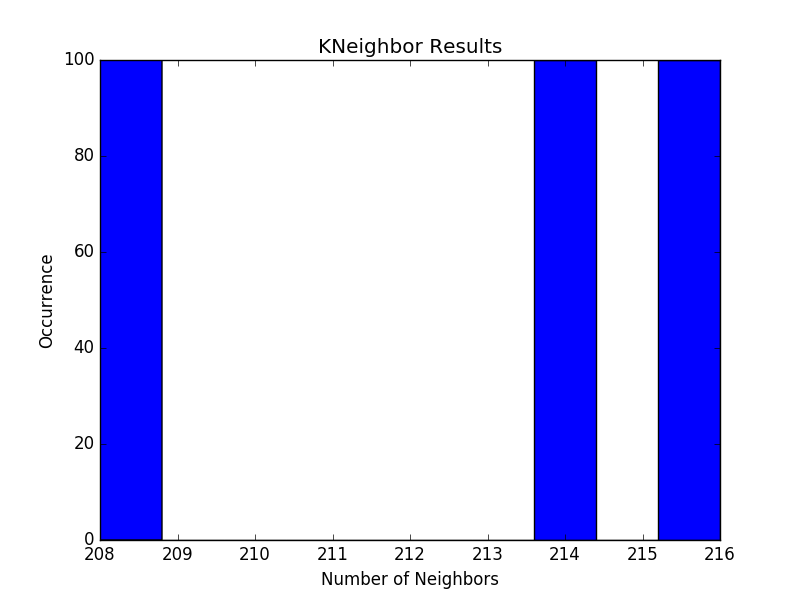
\includegraphics[width=\linewidth]{kneighhistogram.png}
	\caption{Histogram for k-neighbor results.}
\end{figure}

\end{document}